% Present the NN model and the rationale you used to build, train, validate and test it (including the generation of the dataset).

\subsection{Introduction}

The objective is to implement a model based on a Multilayer Neural Network (NN) to control the variation of the Computing Load Percentage (CLPVariation), given some system parameters as input (such as memory, processor, network, etc...).
This neural network should model the Fuzzy System developed in section \ref{sec:fuzzy_system}.


\subsection{Datasets}
The datasets used to build the model were generated using a randomized script and the Fuzzy System previously mentioned.

First, we developed a script to randomize the inputs of the fuzzy system, and then feed them to the fuzzy system to obtain the expected output of the neural network.

To avoid overfitting the model, we must use 3 datasets: Training, Validation and Test.
Instead of generate a mega-dataset and split it, because we wanted to cover the input space uniformly, we decided to generate the datasets independently, knowing that that the points shouldn't overlap in the datasets (that is, there shouldn't be the same inputs in the 3 datasets).

With "cover the input space uniformly" in mind, we decided to generate the points sequentially for the training dataset, to avoid clusters and obtain a balanced dataset. First, we generated numbers using 11 training points for each of the 4 used features \textit{(Processor Load, Memory Usage, Output Throughput and Output Bandwidth)}, generating numbers with a 0.1 interval (between 0 and 1), and randomized the values for the variations and the unused features, as these values wouldn't be used anyway as an input of the model. This created a dataset with $11^{4} = 14 641$ examples.

To validate and test the model, we decided to use truly random values for all the features, so we generated a data set with 10 000 000 points, and split it 50/50, to originate our Validation and Test Datasets.


\subsection{Regression problem}

The neural network is expected to replicate the results of the Fuzzy System. This is a regression problem, as the goal is to predict a quantitative value.


\subsubsection{NN model}

To begin training the model, we used a MLPRegressor model, with the \textit{logistic} activation function and the \textit{sgd} (stochastic gradient descent) solver.
Next, it was needed to tune the parameters and hyperparameters of the model (number of inputs, number of hidden layers, etc), so we developed a script to iterate over them and find the best values.
We started by testing our model by hand for a single hidden layer of 1 to 8 neurons and concluded that 5 neurons gave the lowest \textit{mean squared error} as we can see in Table \ref{tab:MSE_5_log_sgd}.

\begin{table}[H]
    \centering
    \begin{tabular}{l|l|}
        \cline{2-2}
                                       & MSE       \\ \hline
        \multicolumn{1}{|l|}{Validate} & 0.0697423 \\ \hline
        \multicolumn{1}{|l|}{Test}     & 0.07008434  \\ \hline
    \end{tabular}
    \caption{Mean Square Error for 5 neurons with logistic activation and sgd solver}
    \label{tab:MSE_5_log_sgd}
\end{table}

We then used \textit{Grid Search} to optimize the parameters and discovered that this approach yielded improved results. Specifically, we achieved better performance with \textit{activation='relu' and solver='adam'} compared to the original settings of \textit{activation='logistic' and solver='sgd'}.

After that, we tested for combinations of 1 and 2 hidden layers and tested from 1->20 neurons on a single or 2 layers, and we reached the lowest error at 8 neurons on the first layer and 3 neurons on the second.

\begin{verbatim}
    INFO: Best parameters found: {'activation': 'relu', 'alpha': 0.0001,
    'hidden_layer_sizes': (8, 3), 'learning_rate': 'constant', 'max_iter': 2000,
    'solver': 'adam'}
    INFO: Mean Squared Error with best parameters: 0.016218705321498234
\end{verbatim}

From the output of the Grid Search function above, we obtain the final results: 2 hidden layers, the first with 8 nodes, the second with 3, \textit{relu} activation function and the \textit{adam} solver.

We trained our final model (illustrated in Figure \ref{fig:NN_diagram}) using these parameters and the training dataset. With this model, the Mean Squared Error for the validation dataset is 0.0162187.

\begin{figure}[H]
    \centering
    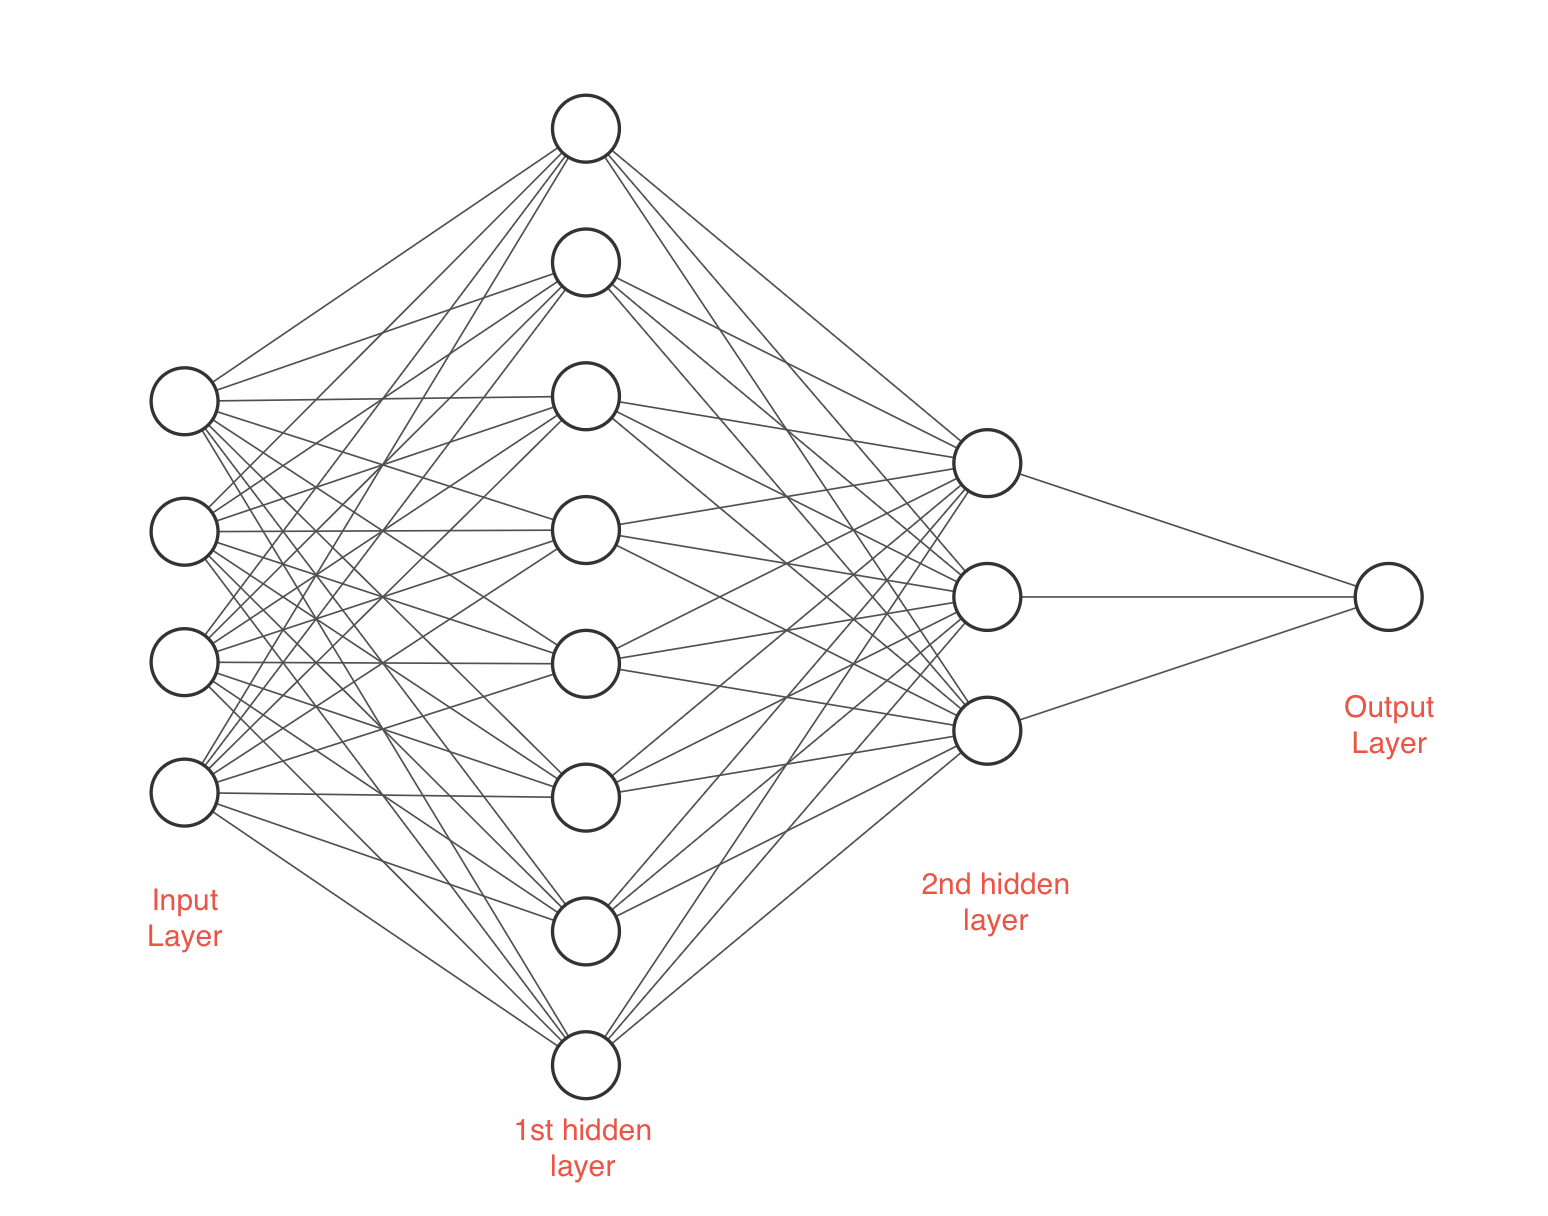
\includegraphics[width=\textwidth]{images/NN_diagram.png}
    \caption{Visual representation of the final Neural Network}
    \label{fig:NN_diagram}
\end{figure}


\subsection{Results}

To evaluate our final model, we tested it against our Test dataset. The results are presented in Table \ref{tab:MSE_11_relu_adam}.

\begin{table}[H]
    \centering
    \begin{tabular}{l|l|}
        \cline{2-2}
                                       & MSE       \\ \hline
        \multicolumn{1}{|l|}{Validate} & 0.0162187 \\ \hline
        \multicolumn{1}{|l|}{Test}     & 0.0162200 \\ \hline
    \end{tabular}
    \caption{Mean Square Error for 8+3 neurons with relu activation and adam solver}
    \label{tab:MSE_11_relu_adam}
\end{table}

The mean squared error (MSE) of the model on the test set is calculated to be 0.0162200. This metric provides insight into the average squared difference between the actual and predicted values. A lower MSE indicates better model performance, with values closer to zero indicating a more accurate prediction. In this case, the MSE suggests that the model's predictions deviate from the actual values by an average squared error of approximately 0.016. We can also see that the 2 values for the errors are very similar, which suggests for once that the two datasets are similarly balanced, and twice that the final model should be a good model (without overfitting), predicting correctly any new value, that it hasn't been "seen" yet.

\begin{figure}[H]
    \centering
    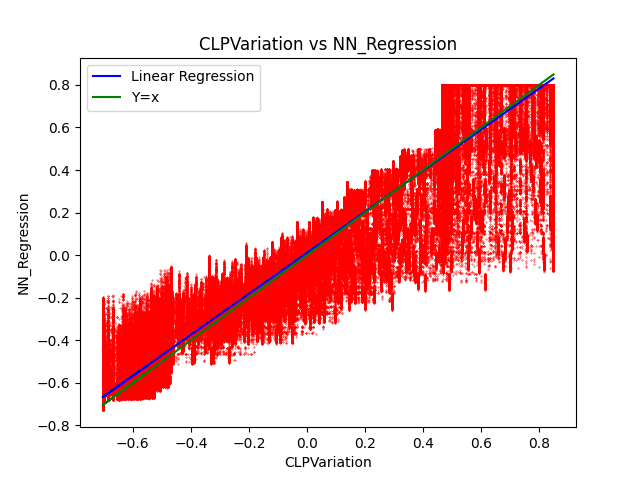
\includegraphics[width=\textwidth]{images/CLP vs Regression.png}\hfill
    \caption{Linear Regression Expected CLP vs Neural Network Prediction}
    \label{fig:FS_NN_LIN_REG}
\end{figure}

Figure \ref{fig:FS_NN_LIN_REG} shows the representation of the linear regression of our model, the green line the regression of a perfect model. We expected the red points to fall near the green line. We can see that that is the case for the most points, given for the compact red areas around the line.
However, we can also see that there are some outliers present, where some red dots deviate from the line on the right of the graph: where the model should predict a very high CLPVariation (> 0.5), is predicting a moderate increase (between 0 and 0.4). Although this might be a concerning issue, because the MSE that we got is so low, we shouldn't be concerned.
In practical terms, this just means that we aren't using the Edge device capabilities to their possible maximum and also aren't contradicting the expected data. This suggests that the edge device should still be able to achieve its purpose effectively. While there may be slight deviations in the predictions, they remain within acceptable bounds, ensuring the continued functionality and reliability of the system.

\newpage

\subsection{Classification problem}
% Increase, decrease or maintain (classes)

We now want to use the NN as a multiclass classifier with the following 3 classes: “Decrease”, “Maintain”, “Increase”.

To achieve that, we created a function (classification function) that maps the CLPVarition values to the 3 classes. The limits for this function are expressed in Table \ref{tab:classifications}.

\begin{table}[H]
    \centering
    \begin{tabular}{|l|l|l|}
        \hline
        Class    & Lower Bound & Upper Bound  \\
        \hline
        Decrease & $-\infty$   & $-0.2$       \\
        \hline
        Maintain & $-0.2$      & $0.2$        \\
        \hline
        Increase & $0.2$       & $\infty$     \\
        \hline
    \end{tabular}
    \caption{Classification Bounds}
    \label{tab:classifications}
\end{table}

For this problem, we ran the NN model against the 3 datasets (Training, Validation and Test), and feed the output from the model to our classification function. To evaluate the results, we also feed the "correct" values to the classification function, and computed the classification metrics.

\subsubsection{Results}

% Key Metrics Explained:
% Precision: The ratio of correctly predicted positive observations to the total predicted positives. High precision indicates a low false positive rate.
% Recall: The ratio of correctly predicted positive observations to the all observations in the actual class. High recall indicates a low false negative rate.
% F1-Score: The weighted average of Precision and Recall. The F1 Score is especially useful when the class distribution is imbalanced.
% Support: The number of actual occurrences of the class in the dataset.

In tables \ref{tab:classification_report_train} through \ref{tab:confusion_matrix_test} are the classification reports (precision, recall, F1-score and accuracy metrics) and the confusion matrices for the 3 datasets, providing a detailed insight into the performance of the neural network model across the three defined classes: 'Decrease', 'Maintain', and 'Increase'.

%%%%%%%%%%%%%%%%TRAIN%%%%%%%%%%%%%%%%%%

\begin{table}[H]
\centering
\begin{tabular}{|l|l:l:l:l|}
\cline{2-5}
\multicolumn{1}{l|}{} & \multicolumn{1}{l|}{Precision} & \multicolumn{1}{l|}{Recall} & \multicolumn{1}{l|}{F1-score} & support               \\
\hline
Decrease              & 0.92                           & 0.95                        & 0.94                          & 5989               \\
\cline{1-1}
Increase              & 1.00                           & 1.00                        & 1.00                          & 7744                \\
\cline{1-1}
Maintain              & 0.60                           & 0.47                        & 0.53                          & 908               \\
\hline
\multicolumn{1}{l}{}  &                                &                             &                               & \multicolumn{1}{l}{}  \\
\hline
accuracy              &                                &                             & 0.95                          & 14641               \\
\cline{1-1}
macro avg             & 0.84                           & 0.81                        & 0.82                          & 14641               \\
\cline{1-1}
weighted avg          & 0.94                           & 0.95                        & 0.95                          & 14641               \\
\hline
\end{tabular}
    \caption{Classification Report for Training dataset}
    \label{tab:classification_report_train}
\end{table}

\begin{table}[H]
\centering
\begin{tabular}{|cc|c:c:c|} 
\cline{3-5}
\multicolumn{1}{c}{}               &          & \multicolumn{3}{c|}{Predicted}                                          \\
\multicolumn{1}{c}{}               &          & \multicolumn{1}{c}{Decrease} & \multicolumn{1}{c}{Increase} & Maintain  \\ 
\hline
\multirow{3}{*}{Actual} & Decrease & 5703                         & 0                            & 286       \\ 
\cdashline{3-5}
                                   & Increase & 0                            & 7744                         & 0         \\ 
\cdashline{3-5}
                                   & Maintain & 478                          & 0                            & 430       \\
\hline
\end{tabular}
\caption{Confusion Matrix for Training dataset}
    \label{tab:confusion_matrix_train}
\end{table}

The classification report for the training set, summarized in table \ref{tab:classification_report_train}, demonstrates exceptional performance in predicting the 'Decrease' and 'Increase' classes, with precision and recall values both around 0.92 and 1.00 respectively. This indicates that the model is highly accurate in identifying instances where the output is either 'very negative' or 'very positive', with zero false-positives and false-negatives in the 'Increase' class.
This is expected, as this is the dataset used for training the Neural Network, where the weighs are computed to be the very best to meet the excepted output.

%%%%%%%%%%%%%%%%VALIDATE%%%%%%%%%%%%%%%
\begin{table}[H]
\centering
\begin{tabular}{|l|l:l:l:l|}
\cline{2-5}
\multicolumn{1}{l|}{} & \multicolumn{1}{l|}{Precision} & \multicolumn{1}{l|}{Recall} & \multicolumn{1}{l|}{F1-score} & support               \\
\hline
Decrease              & 0.98                           & 0.97                        & 0.97                          & 1859972               \\
\cline{1-1}
Increase              & 0.98                           & 0.98                        & 0.98                          & 2825928                \\
\cline{1-1}
Maintain              & 0.68                           & 0.74                        & 0.71                          & 314100               \\
\hline
\multicolumn{1}{l}{}  &                                &                             &                               & \multicolumn{1}{l}{}  \\
\hline
accuracy              &                                &                             & 0.96                          & 5000000               \\
\cline{1-1}
macro avg             & 0.88                           & 0.90                        & 0.89                          & 5000000               \\
\cline{1-1}
weighted avg          & 0.96                           & 0.96                        & 0.96                          & 5000000               \\
\hline
\end{tabular}
    \caption{Classification Report for Validation dataset}
    \label{tab:classification_report_validate}
\end{table}

\begin{table}[H]
\centering
\begin{tabular}{|cc|c:c:c|} 
\cline{3-5}
\multicolumn{1}{c}{}               &          & \multicolumn{3}{c|}{Predicted}                                          \\
\multicolumn{1}{c}{}               &          & \multicolumn{1}{c}{Decrease} & \multicolumn{1}{c}{Increase} & Maintain  \\ 
\hline
\multirow{3}{*}{Actual} & Decrease & 1794895                        & 0                               & 65077       \\ 
\cdashline{3-5}
                                   & Increase & 211                            & 2782793                         & 42924         \\ 
\cdashline{3-5}
                                   & Maintain & 33844                          & 47120                           & 233136       \\
\hline
\end{tabular}
\caption{Confusion Matrix for Validation dataset}
    \label{tab:confusion_matrix_validate}
\end{table}

%%%%%%%%%%%%%%%%TEST%%%%%%%%%%%%%%%%%%%
\begin{table}[H]
\centering
\begin{tabular}{|l|l:l:l:l|}
\cline{2-5}
\multicolumn{1}{l|}{} & \multicolumn{1}{l|}{Precision} & \multicolumn{1}{l|}{Recall} & \multicolumn{1}{l|}{F1-score} & support               \\
\hline
Decrease              & 0.98                           & 0.96                        & 0.97                          & 1858190               \\
\cline{1-1}
Increase              & 0.98                           & 0.98                        & 0.98                          & 2827993                \\
\cline{1-1}
Maintain              & 0.68                           & 0.74                        & 0.71                          & 313817               \\
\hline
\multicolumn{1}{l}{}  &                                &                             &                               & \multicolumn{1}{l}{}  \\
\hline
accuracy              &                                &                             & 0.96                          & 5000000               \\
\cline{1-1}
macro avg             & 0.88                           & 0.90                        & 0.89                          & 5000000               \\
\cline{1-1}
weighted avg          & 0.96                           & 0.96                        & 0.96                          & 5000000               \\
\hline
\end{tabular}
    \caption{Classification Report for Test dataset}
    \label{tab:classification_report_test}
\end{table}

\begin{table}[H]
\centering
\begin{tabular}{|cc|c:c:c|} 
\cline{3-5}
\multicolumn{1}{c}{}               &          & \multicolumn{3}{c|}{Predicted}                                          \\
\multicolumn{1}{c}{}               &          & \multicolumn{1}{c}{Decrease} & \multicolumn{1}{c}{Increase} & Maintain  \\ 
\hline
\multirow{3}{*}{Actual} & Decrease & 1792873                        & 0                               & 65317       \\ 
\cdashline{3-5}
                                   & Increase & 250                            & 2784752                         & 42991         \\ 
\cdashline{3-5}
                                   & Maintain & 33923                          & 47101                           & 232793       \\
\hline
\end{tabular}
    \caption{Confusion Matrix for Test dataset}
    \label{tab:confusion_matrix_test}
\end{table}

Because the Validation and Test datasets share the same results, they are analysed together.
Both for the Validation and Test dataset, it is observed a high precision, recall and F1-score for the "Decrease" and "Increase" classes, with values between 0.96 and 0.98. However, the model's performance for the 'Maintain' class is notably lower, with a precision of 0.68 and recall of 0.74, resulting in an F1-score of 0.71 (for the 2 datasets). This suggests that the model has difficulty distinguishing instances where the output is closer to 0, leading to a higher rate of misclassification in this category. This discrepancy is likely due to the class imbalance in the dataset, where the 'Maintain' class has significantly fewer samples compared to the 'Decrease' and 'Increase' classes.

The overall accuracy of the model stands at 96\%, which indicates that the majority of the predictions are correct. The macro average metrics, which treat all classes equally, show slightly lower values (precision: 0.88, recall: 0.90, F1-score: 0.89), reflecting the model's challenges with the 'Maintain' class. In contrast, the weighted average metrics, which consider the number of instances per class, align closely with the high overall accuracy, as the performance on the dominant classes ('Decrease' and 'Increase') heavily influences these averages.

Additionally, the confusion matrix for the Test dataset, as shown in table \ref{tab:confusion_matrix_test}, further illustrates the model's performance by summarizing the number of correct and incorrect predictions for each class. The confusion matrix reveals that the model accurately predicts the 'Decrease' and 'Increase' classes, with a large number of true positive predictions (1,792,873 and 2,784,752, respectively) and relatively low false positive and false negative predictions. However, the model struggles more with the 'Maintain' class, as evidenced by the higher number of false positive and false negative predictions compared to the other classes. These insights from the confusion matrix help identify areas for improvement and guide future refinements to enhance the model's predictive capabilities.
